\documentclass[11pt]{article}
\usepackage{amsmath, amssymb}
\usepackage{geometry}
\geometry{margin=1in}
\usepackage{fancyhdr}
\usepackage{lastpage}
\usepackage{parskip} % Better paragraph spacing
\usepackage{titlesec} % Better section formatting
\usepackage{graphicx}
\usepackage{float}
\usepackage[most]{tcolorbox}
\usepackage{lmodern}
\usepackage{caption}
\usepackage{hyperref}
\usepackage{listings}
\usepackage{xcolor}

\definecolor{codegreen}{rgb}{0,0.6,0}
\definecolor{codegray}{rgb}{0.5,0.5,0.5}
\definecolor{codepurple}{rgb}{0.58,0,0.82}
\definecolor{backcolour}{rgb}{0.95,0.95,0.92}

% Define code styling
\lstdefinestyle{mystyle}{
    backgroundcolor=\color{backcolour},
    commentstyle=\color{codegreen},
    keywordstyle=\color{magenta},
    numberstyle=\tiny\color{codegray},
    stringstyle=\color{codepurple},
    basicstyle=\ttfamily\footnotesize,
    breakatwhitespace=false,
    breaklines=true,
    captionpos=b,
    keepspaces=true,
    numbers=left,
    numbersep=5pt,
    showspaces=false,
    showstringspaces=false,
    showtabs=false,
    tabsize=2
}

\lstset{style=mystyle}

% Define commands for reusable content
\newcommand{\coursename}{COM-407 Advanced Networks}
\newcommand{\lecturenum}{08}
\newcommand{\lecturedate}{07/11/2025§}
\newcommand{\professor}{Pavlos Nikopoulous}

\hypersetup{colorlinks=true,linkcolor=blue,urlcolor=blue}

% Configure section spacing
\titlespacing*{\section}{0pt}{2ex plus 1ex minus .2ex}{1.5ex plus .2ex}
\titlespacing*{\subsection}{0pt}{1.5ex plus 1ex minus .2ex}{1ex plus .2ex}
% Header / Footer
\pagestyle{fancy}
\fancyhf{}
\fancyhead[L]{\coursename}
\fancyhead[R]{Lecture \lecturenum}
\fancyfoot[L]{EPFL - Computer Science}
\fancyfoot[C]{Author: Jonathan Dutoit}
\fancyfoot[R]{Page \thepage\ of \pageref{LastPage}}

\begin{document}

\begin{center}
  {\large EPFL - Computer Science} \\[0.5em]
  {\Large \textbf{\coursename}} \\[0.5em]
  {\large Lecture \lecturenum\ --- \lecturedate} \\[0.5em]
  {\large Author: Jonathan Dutoit} \\[0.5em]
  {\large Professor: \professor} \\[0.5em]
\end{center}

\vspace{2cm}
\begin{center}
  {\LARGE \textbf{Transport Layer Continued}}
\end{center}

\vspace{1cm}


\section*{TCP Fast Open (TFO)}

\textcolor{red}{Why?} Avoid latency of 3-way handshake when re-opening repeated connections

\textcolor{red}{How?}
\begin{itemize}
	\item Server includes in \textcolor{blue}{\textit{TCP options}} of SYN-ACK a \textcolor{blue}{\textit{message authentication code (MAC)}}: \\
	t = \verb|crypto_hash(k, c)| 
	\begin{itemize}
		\item k is a secret, unknown to client
		\item c is the client's IP address
	\end{itemize}
	\item Client caches \textit{t}
	\item Uses it when opening next connection
		\begin{itemize}
			\item Client sends back \textit{t} within SYN packet
	\item After receiving SYN and \textit{t}, server knows that "this client has connected earlier"
	\item Server can send \textit{\textcolor{red}{data within SYN-ACK}}
\end{itemize}
\end{itemize}
% Quick centered image
\begin{figure}[H]
    \centering
    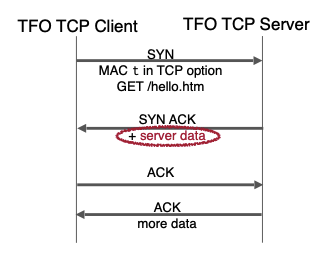
\includegraphics[width=0.4\textwidth]{images/tfo}
    \label{fig:LABEL}
\end{figure}

\newpage
\section*{5. Secure Transport}

\begin{itemize}
	\item TCP is not secure
	\item can be secured with a security sub-layer:
		\begin{itemize}
			\item $\rightarrow$ Transport Layer Security (TLS)
		\end{itemize}
	\item TLS adds to TCP: \textcolor{red}{confidentiality} (data is encrypted) and \textcolor{red}{authentication} (data is protected against forgery)
\end{itemize}
% Quick centered image
\begin{figure}[H]
    \centering
    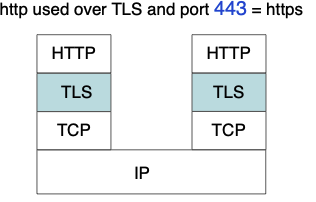
\includegraphics[width=0.4\textwidth]{images/http}
    \label{fig:LABEL}
\end{figure}

\section*{TLS 1.3}

\begin{minipage}{0.6\textwidth}
\begin{itemize}
	\item does not support RSA key exchange \\
	\item Communicating parties:
		\begin{itemize}
			\item agree on cryptographic suites \\
			\item exchange cryptographic parameters to compute session keys ($\sim$ "\textcolor{red}{Diffie-Hellman}" approach) \\
		\end{itemize}
	\item needs \textit{\textcolor{blue}{1-RTT handshake}} before sending application data \\
\end{itemize}
\end{minipage}
\hfill
\begin{minipage}{0.4\textwidth}
\centering
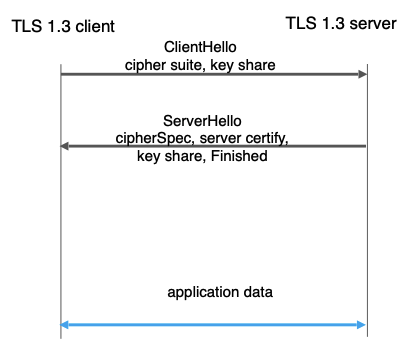
\includegraphics[width=\linewidth]{images/tls}
\end{minipage}

\section*{TLS Sockets}

TLS sockets (also called SSL sockets) are transformed/"\textcolor{blue}{\textit{wrapped}}" sockets. 

% Quick centered image
\begin{figure}[H]
    \centering
    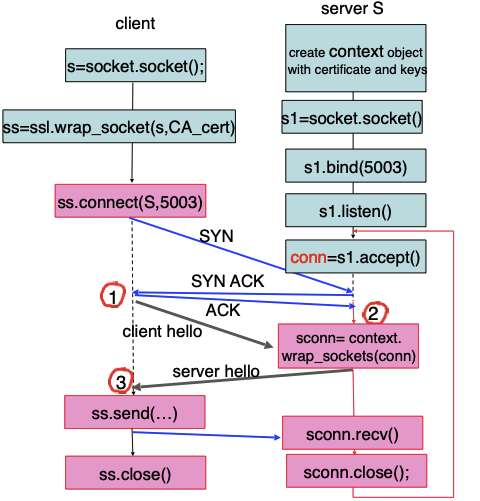
\includegraphics[width=0.5\textwidth]{images/tls-sockets}
    \label{fig:LABEL}
\end{figure}

\begin{tcolorbox}[
  colback=gray!15,     % background color
  colframe=black!50,    % border color
  boxrule=1pt,       % border thickness
  arc=3mm,             % rounded corners
  left=4mm, right=4mm, top=2mm, bottom=2mm % padding
]
\textbf{With https/TLS1.3, how many RTTs are required before data transfer can occur?}

\vspace{0.3cm}

A. 1 \\
B. 2 \\
C. 3 \\
D. 4 \\
E. 0 \\
F. I don't know \\

\textbf{Answer}: B. 1 RTT for opening the TCP connection and 1 RTT (at least) for establishing the TLS session
\end{tcolorbox}

\newpage
\begin{center}
  {\LARGE \textbf{IP Multicast}}
\end{center}

\vspace{1cm}
\begin{itemize}
	\item Recall:
		\begin{itemize}
			\item Unicast = source sends data to a \textcolor{blue}{\textit{unicast}} IP address, and a \textcolor{blue}{\textit{single}} destination receives it
			\item Multicast = source sends data to a \textcolor{red}{\textit{multicast}} IP address, but \textcolor{red}{\textit{multiple}} destination receive it
		\end{itemize}
	\item Multicast delivers the same data to multiple recipients \textcolor{blue}{\textit{without}} sending multiple copies from the source\\
	$\rightarrow$ Traffic is \textcolor{purple}{\textit{replicated}} at the \textit{\textcolor{purple}{network layer}}
	\item Used only:
		\begin{itemize}
			\item with \textcolor{red}{\textit{UDP}} (cannot be done with TCP!)
			\item within a \textcolor{red}{\textit{single domain}} (= network belonging to a single administrative entity, composed of multiple subnets)
		\end{itemize}
\end{itemize}

% Quick centered image
\begin{figure}[H]
    \centering
    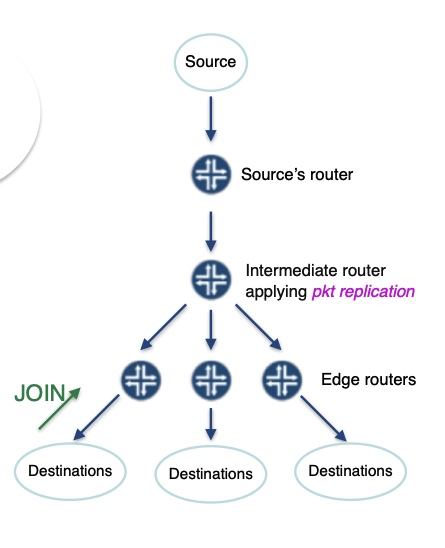
\includegraphics[width=0.4\textwidth]{images/ip-multicast}
    \label{fig:LABEL}
\end{figure}
\subsection*{Typical process}

\begin{enumerate}
	\item Destination \textit{\textcolor{green}{subscribe to}} a multicast group by sending \textit{\textcolor{green}{join}} messages to their gateway routers
		\begin{itemize}
			\item IGMP (Internet Group Management Protocol, in IPv4)
			\item MLD (Multicast Listener Discovery, in IPv6)
		\end{itemize}
	\item Routers either build distribution tree (PIM) or use a \textcolor{red}{\textit{tunneling}} approach (BIER)
	\item Source sends packets to multicast address
	\item Intermediate IP routers between source and destinations \textit{\textcolor{purple}{replicate traffic}}
\end{enumerate}

\section*{Multicast addresses and groups}

\begin{minipage}{0.6\textwidth}
\begin{itemize}
	\item Reserved address spaces:
		\begin{itemize}
			\item IPv4: \textbf{224.0.0.0/4} (i.e. 224.0.0.0 to 239.255.255.255)
			\item IPv6: \textbf{ff00::/8}, bits 13-16 determine the "scope": \\
			ff02/16 = same subnet, \\
			ff05/16 = same domain \\
		\end{itemize}
	\item \textcolor{blue}{\textit{Any Source Multicast}} (ASM) group:
		\begin{itemize}
			\item identified by the multicast address;
			\item \textcolor{red}{\textit{any}} source can send to this group \\
		\end{itemize}
	\item \textcolor{blue}{\textit{Source Specific Multicast}} (SSM) group:
		\begin{itemize}
			\item identified by \textcolor{blue}{\texttt{(s, m)}} \\
			where \textit{\textbf{m}} is a multicast address and \textbf{\textit{s}} is a (unicast) source IP address;
			\item \textcolor{red}{\textit{only}} \textbf{\textit{s}} can send to this group; OS discards packets from irrelevant sources
			\item default SSM addresses: 232.0.0.0/8, ff3x::/96 (x=scope bits; e.g., ff35::/96 = site-local)
			
		\end{itemize}
\end{itemize}

\end{minipage}
\hfill
\begin{minipage}{0.4\textwidth}
\centering
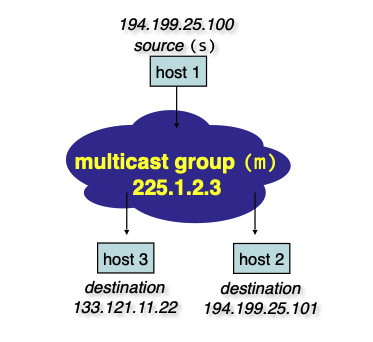
\includegraphics[width=\linewidth]{images/multicast-addresses}
\end{minipage}

\section*{PIM: Protocol Independent Multicast}
% Quick centered image
\begin{figure}[H]
    \centering
    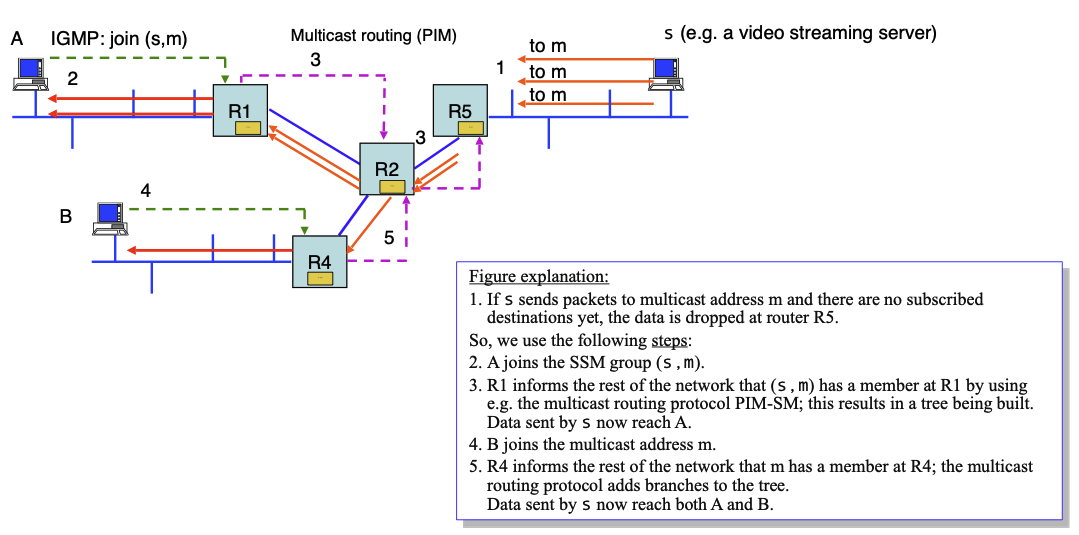
\includegraphics[width=1\textwidth]{images/PIM}
    \label{fig:LABEL}
\end{figure}


PIM supports ASM and SSM. Exists in 2 versions:
\begin{itemize}
	\item PIM-DM (\textit{\textcolor{blue}{Dense}} Mode): heavy use of broadcast, used only in small networks
	\item PIM-SM (\textcolor{blue}{\textit{Sparse}} Mode): widespread, used e.g., for TV distribution
		\begin{itemize}
			\item If used for SSM, PIM-SM uses \textcolor{red}{\textit{reverse path forwarding (RPF)}}
			\item This creates the distribution tree \textit{\textcolor{blue}{on the fly}}
		\end{itemize}
\end{itemize}

\subsection*{PIM routers keep per-(multicast)-flow state}
In addition to longest prefix match, PIM routers keep state for multicast groups and apply \textit{\textcolor{blue}{exact-match}} lookup. 
% Quick centered image
\begin{figure}[H]
    \centering
    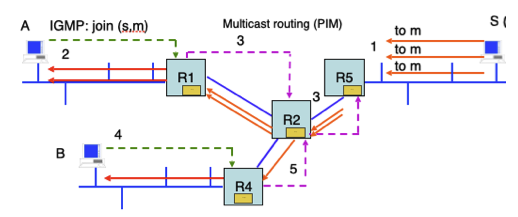
\includegraphics[width=0.6\textwidth]{images/pim-2}
    \label{fig:LABEL}
\end{figure}

Multicast \textcolor{red}{\textit{state information}} is dynamically kept in router for every known multicast group: 
\begin{itemize}
	\item \textit{(s, m) or (*, m)} $\rightarrow$ id of group 
	\item \textit{valid incoming interfaces} $\rightarrow$ for security
	\item \textit{outgoing interfaces} $\rightarrow$ this is the forwarding info
	\item \textit{other information required by multicast routing protocol}
\end{itemize}

\section*{BIER (Bit Index Explicit Replication)}

\textbf{Why?} \\
Per-flow state is \textit{dynamic} (depends on who listens to the group) and \textit{cannot} be aggregated based on prefix \\
$\rightarrow$ \textcolor{red}{\textit{Scalability issues}} at backbone routers; state info may be significantly large. 

\textbf{What?}
\begin{itemize}
	\item Keep \textit{\textbf{no}} state at backbone routers; put forwarding info \textit{\textcolor{blue}{inside}} packets ($\sim$tunneling)
		\begin{itemize}
			\item Every multicast packet has an \textcolor{blue}{\textit{extension header}} carrying the list of destination routers (a.k.a. Bit-Forwarding Egress Routers, BFERs)
			\item Routers use packet's header and their forwarding table to multicast packets:
				\begin{itemize}
					\item for \textit{\textcolor{blue}{all}} BFERs in header reached through the same next hop, only a \textcolor{blue}{\textit{single}} copy is create
					\item in this copy, the BIER header is modified accordingly
				\end{itemize}
		\end{itemize}
\end{itemize}

% Quick centered image
\begin{figure}[H]
    \centering
    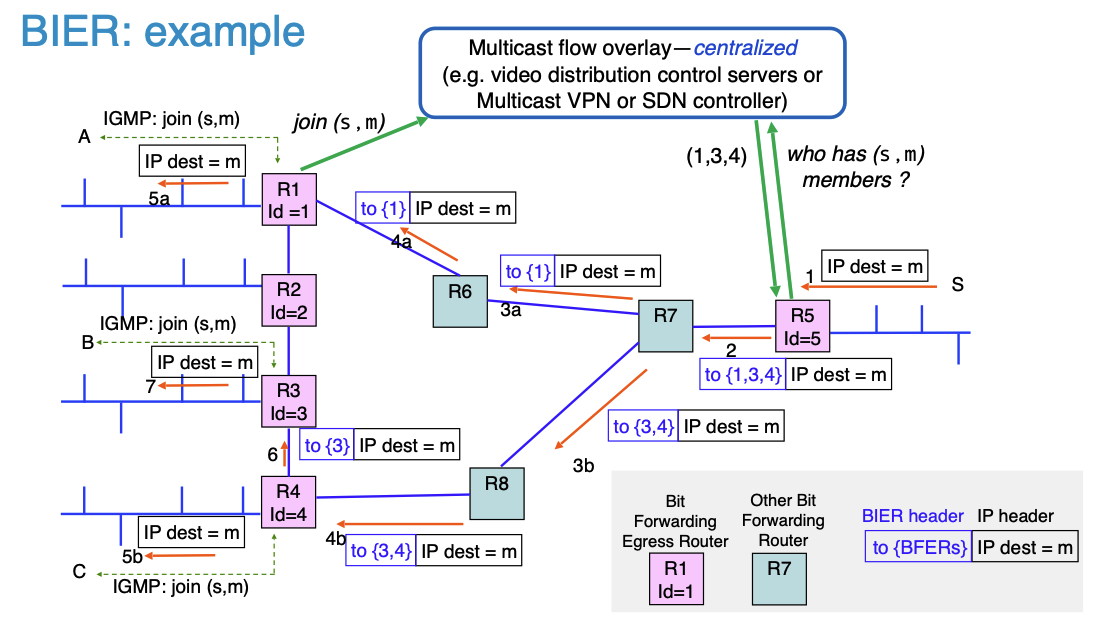
\includegraphics[width=1\textwidth]{images/bier}
    \label{fig:LABEL}
\end{figure}

\subsection*{BIER: Packet replication and forwarding}

\begin{minipage}{0.6\textwidth}
\begin{itemize}
	\item For each destination BFER, BIER router pre-computes (based on the IP forwarding table) a \textcolor{purple}{"forwarding bit mask"} that indicates the set of destination BFERs that are \textcolor{blue}{reached} by the same next-hop \\
	\item To forwarding a packet, with destination set \textit{S}, BIER router runs: \\
	\begin{enumerate}
		\item \texttt{Send a copy to 1st destination in S with destination set = $S \cap S_1$, where $S_1$ is the forwarding bit mask of 1st destination.}
		\item \texttt{If $S \backslash S_1 \neq \emptyset$, duplicate the packet but with destination $S \backslash S_1$ and goto 1; else break.}
	\end{enumerate}
\end{itemize}

\end{minipage}
\hfill
\begin{minipage}{0.4\textwidth}
\centering
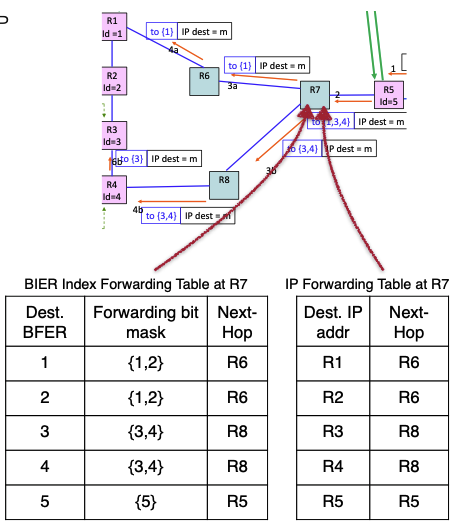
\includegraphics[width=\linewidth]{images/bier-algo}
\end{minipage}
\begin{tcolorbox}[
  colback=gray!15,     % background color
  colframe=black!50,    % border color
  boxrule=1pt,       % border thickness
  arc=3mm,             % rounded corners
  left=4mm, right=4mm, top=2mm, bottom=2mm % padding
]
\textbf{Example at router r7} \\
R7 receives packet with destination set \texttt{S = \{1,3,4\}}
\begin{enumerate}
\item First destination in \textit{S} is 1, R7 uses Bier Index Forwarding table and finds that the forwarding bit mask for destination 1 is $S_1 = \{1,2\}$: sends a copy of packet to next-hop (R6) with destination $S' = S \cap S_1 = \{1\}$
\item $S''= S \backslash \{1, 2\} = \{3, 4\}$ is not empty; R7 duplicates packet with destination $S''$ and applies the same: first destination is 3, so R7 sends a copy to next-hop (R8) with destination set $\{3, 4\}$
\item Now $\{3,4\} \backslash \{3, 4\} = \emptyset$, so it breaks.
\end{enumerate}
\end{tcolorbox}

\subsection*{How to optimize processing at BIER routers?}
\begin{itemize}
	\item BIER routers encode the forwarding bit masks and destination sets into \textcolor{red}{\textit{bitstrings}}. E.g. with 5 BFERs:
		\begin{itemize}
			\item Destination BFERs = $\{1,3,4\} \rightarrow$ bitstring $ = 01101$
			\item  Destination BFERs = $\{3,4\} \rightarrow$ bitstring $ = 01100$
			\item  Destination BFERs = $\{1\} \rightarrow$ bitstring $ = 00001$	
		\end{itemize}
		
	\item Set intersection becomes a \textcolor{blue}{\textit{bitwise AND with mask}}
	\item Set difference becomes a \textcolor{blue}{\textit{bitwise AND with the bit-inverted mask}}
	\item More complicated mechanisms exit, if the number of BFERs is large
\end{itemize}

\section*{BIER - recap}
\begin{minipage}{0.6\textwidth}
\begin{itemize}
	\item Routers have 2 tables:
		\begin{itemize}
			\item Unicast IP forwarding table (longest prefix match)
			\item Bit Index Forwarding table is automatically derived from unicast IP forwarding table (exact match); stores no per-flow state
		\end{itemize}
	\item apply \textcolor{red}{\textit{bistring processing}} using a 
	\item Bit Forwarding Ingress Router (BFIR, such as R5) caches mappings of multicast addresses to BIER headers
		\begin{itemize}
			\item needs to access an \textcolor{blue}{\textit{out of band, centralized entity}};
			\item this is the \textcolor{blue}{\textit{only}} (dynamic) per-flow state kept in BIER
		\end{itemize}
	\item Multicast packets are forwarded based on BIER header, destination IP address is not used ($\sim$\textcolor{red}{\textit{tunneling}})
\end{itemize}

Multiple BIER domains can be interconnected by BFIR-BFER interconnection
\end{minipage}
\hfill
\begin{minipage}{0.4\textwidth}
\centering
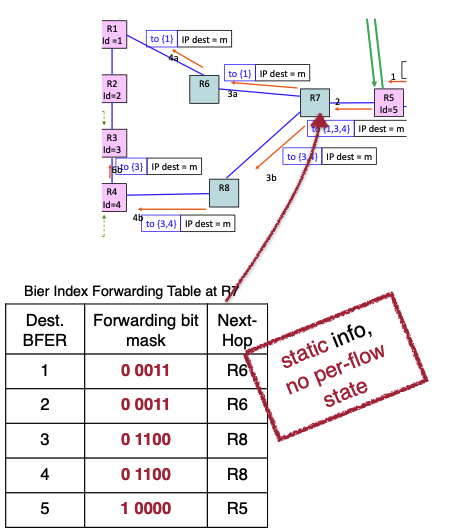
\includegraphics[width=\linewidth]{images/bier-recap}
\end{minipage}

\section*{Is there Multicast ARP (address resolution protocol)?}
\begin{minipage}{0.6\textwidth}
\begin{itemize}
	\item \textcolor{red}{\textit{No}}, multicast MAC address is \textcolor{blue}{\textit{algorithmically}} derived from multicast IP adress:
		\begin{itemize}
			\item Last 23 bits of IPv4 multicast address are used in MAC addresses
			\item Last 32 bits of IPv6 multicast address are used in MAC addresses \\
		\end{itemize}
	\item Notes:
		\begin{itemize}
			\item Multicast MAC depends only on multicast IP address \textit{m}, not on source address \textit{s}, even if \textit{m} is an SSM address
			\item Several multicast IP addresses may yield the same MAC
			\begin{itemize}
				\item packets received unnecessarily at the MAC layer are removed by the OS; hopefully this happens rarely
			\end{itemize}
		\end{itemize}
\end{itemize}

\end{minipage}
\hfill
\begin{minipage}{0.4\textwidth}
\centering
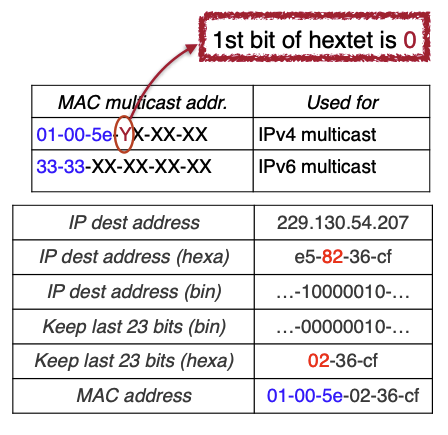
\includegraphics[width=\linewidth]{images/multicast-arp}
\end{minipage}

\section*{MAC Multicast: how do switches handle multicast frames?}
% Quick centered image
\begin{figure}[H]
    \centering
    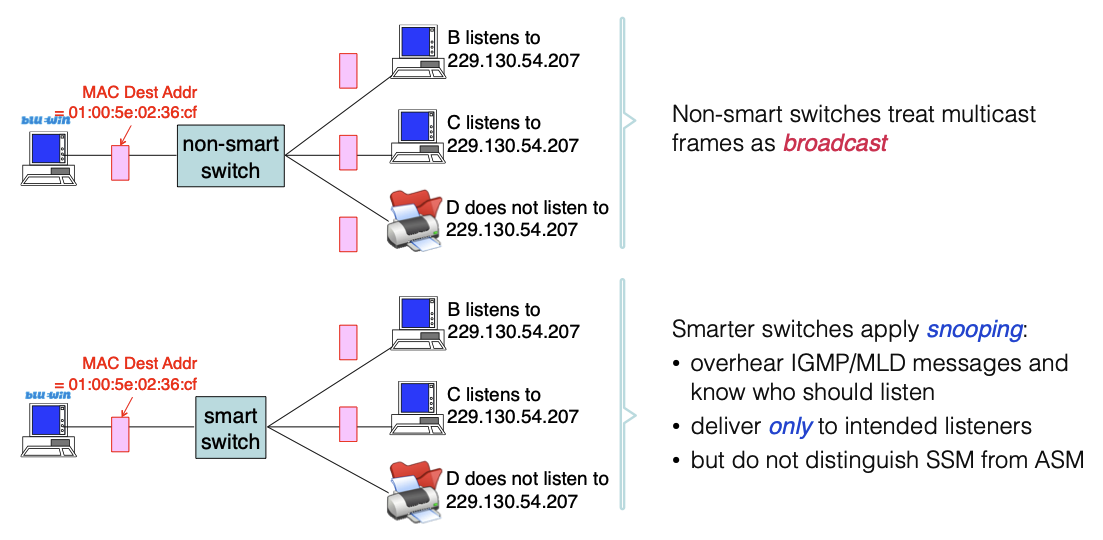
\includegraphics[width=1\textwidth]{images/multicast-switches}
    \label{fig:LABEL}
\end{figure}

\section*{Security of IP Multicast}

IP multicast w/ or w/o BIER makes attacks easier (e.g., \textcolor{red}{\textit{Denial of Service}}, witty worm). Mitigations: limit multicast rate and number of groups; control which multicast group is allowed (\textcolor{blue}{\textit{access lists}})


SSM is safer because routers and destination can reject misbehaving sources

IGMP/MLD is not secure and has the same problems as ARP/NDP. Mitigated by same mechanisms: sniffing switches observe all traffic and implement \textcolor{blue}{\textit{access control}}

Multicast-capable networks must deploy exhaustive \textcolor{blue}{\textit{filtering}} and \textcolor{blue}{\textit{monitoring}} tools to limit potential damage.

\section*{Multicast in Practice}
\begin{itemize}
	\item Multicast is good for \textcolor{red}{sources}: one packet sent for \textbf{\textit{n}} destinations -- replication is done \textbf{\textit{O(log(n))}} times
	\item Multicast is not supported everywhere, but is used in:
		\begin{itemize}
			\item Internet TV distribution (PIM-SM / BIER)
			\item EPFL and other academic networks (PIM-SM)
			\item Data Center Virtualization Services (BIER)
			\item Some corporate networks for news, sensor streaming, time synchronization, large videoconferences, etcs...
			\item Industrial networks (smart grids, factory automation)
		\end{itemize}
	\item Works only with \textcolor{red}{UDP}, not with TCP (not easy to handle TCP acks from multiple receivers, the goal of multicast would be defeated) $\rightarrow$ need to handle \textcolor{red}{errors}, usually via redundancy (extra traffic)
\end{itemize}

\end{document}
